\documentclass[a4paper]{article}
\usepackage[utf8]{inputenc}
\usepackage[russian]{babel}
\usepackage[T2]{fontenc}
\usepackage[warn]{mathtext}
\usepackage{graphicx}
\usepackage{amsmath}
\usepackage{floatflt}
\usepackage[left=20mm, top=20mm, right=20mm, bottom=20mm, footskip=10mm]{geometry}


\graphicspath{ {images/} }
\usepackage{multicol}
\setlength{\columnsep}{2cm}


\begin{document}

\begin{titlepage}
	\centering
	\vspace{5cm}
	{\scshape\LARGE Московский физико-технический институт \par}
	\vspace{4cm}
	{\scshape\Large Лабораторная работа \par}
	\vspace{1cm}
	{\huge\bfseries Опыт Милликена \par}
	\vspace{1cm}
	\vfill
\begin{flushright}
	{\large выполнила студентка 653 группы ФФКЭ}\par
	\vspace{0.3cm}
	{\LARGE Карпова Татьяна}
\end{flushright}
	

	\vfill

% Bottom of the page
	Долгопрудный, 2017 г.
\end{titlepage}

\section{Цель работы}
Определение заряда электрона методом масляных капель

\section{В работе используются:}
\begin{itemize}
    \item плоский конденсатор в защитном кожухе
    \item осветитель
    \item измерительный микроскоп
    \item электростатический вольтметр
    \item электронный секундомер
    \item переключатель напряжения
    \item пульверизатор с маслом
\end{itemize}

\section{Теоретические положения}

Если заряд действительно существует, то заряд любого тела может принимать дискретную последовательность значений $\pm e, \pm 2e, \pm 3e ...$ \par
Рассматривая движение капли в гравитационном поле с учётом электростатических сил и сил трения:
\begin{equation}
    q= 9 \pi \sqrt{\frac{2\eta^3 h^3}{g\rho}}\frac{l(t_0 + t)}{V t_0^{3/2}t},
\end{equation}
где $\eta = 1,85*10^{-5}$Па*с - вязкость воздуха, $h = 0.25$ мм - расстояние, пройденное каплей, $\rho = 898$ кг/см$^3$ - вязкость масла, $t_0$ - время свободного падения капли, $t$ - время подъёма капли в конденсаторе, $V$ - напряжение на конденсаторе. \par
Погрешность измерения заряда определяется по формуле 
\begin{equation}
    \sigma_q = q\sqrt{(\frac{\sigma_V}{V})^2 + (\frac{\sigma_t t_0}{t(t_0 + t)})^2 + (\frac{\sigma_t_0(3t + t_0)}{2t_0(t+t_0)})^2}
\end{equation}

\section{Экспериментальная установка}

\begin{figure}[h]
    \centering
    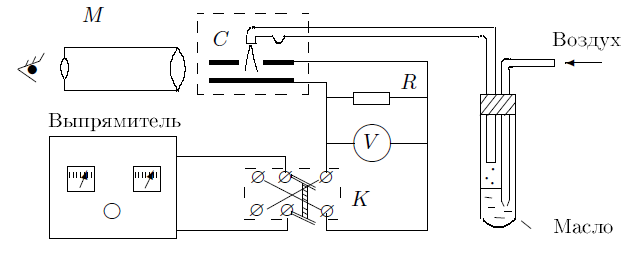
\includegraphics[width=10cm]{fig1.PNG}
    \caption{Схема установки для измерения заряда электрона}
    \label{fig:vac}
\end{figure}

Масло разбрызгивается пульверизатором. Капли масла попадают в конденсатор С через небольшое отверстие в верхней пластине. При этом часть из них вследствие трения о воздух приобретает случайный по знаку и модулю электрический заряд. Напряжение подаётся с регулируемого выпрямителя и измеряется вольтметром V. С помощью ключа К можно менять направление поля в конденсаторе, чтобы можно было работать как с положительно, так и с отрицательно заряженными каплями.

\section{Ход работы}

\begin{enumerate}
    \item Подготовим установку к работе, проведём пробные измерения. 
    \item Для 14 капель будем замерять время её свободного падения $t_0$ и время подъёма в поле конденсатора $t$. Результаты занесём в таблицу 2
    
    \begin{table}[h]
    \centering
    \begin{center}
    \caption{Заряды капель}
    \end{center}
    \vspace{0.1cm}
    \label{tab:my_label}
    \begin{tabular}{ |p{2cm}||p{1.2cm}|p{1.2cm}|p{1.2cm}|p{1.cm}|p{1.2cm}|p{1.2cm}|p{1.2cm}| }
 \hline
    $q, 10^{-19}$Кл & 1.305 & 3.475 & 1.508 & 1.481 & 2.623 & 1.477 & 1.578 \\
\hline
    $q/e$ & 0.815 & 2.172 & 0.942 & 0.926 & 1.639 & 0.923 & 0.987\\
     
\hline
 \hline
    $q, 10^{-19}$Кл & 1.416 & 2.765 & 1.769 & 1.743 & 1.486 & 1.647 &  \\
\hline
    $q/e$ & 0.885 & 1.728 & 1.106 & 1.090 & 0.929 & 1.029 & \\

     
\hline
\hline
    

    \end{tabular}
\end{table}
    
      \begin{table}[h]
    \centering
    \begin{center}
    \caption{Движение капель свободное и в поле конденсатора}
    \end{center}
    \vspace{0.1cm}
    \label{tab:my_label}
    \begin{tabular}{ |p{1cm}||p{2cm}|p{3cm}|p{2cm}|p{1.8cm}|p{2cm}|p{1.8cm}| }
 \hline
    $t_0$, с & 19.46 & 17.6 & 15.12 & 20.3 & 16.17 & $\overline t_0 = $17.73 \\
\hline
    $t$, c & 6.75 & 4.77 & 3.74 & 2.47 & 1.97 & $\overline t = $3.94\\
\hline
     & $V = 540$ кВ & $q_1 = 1.305*10^{-19}$ Кл & $q_1/e$ = 0.815 & $\sigma_q = 0.06$ & $\epsilon_q = 4.61 \%$ &  \\
     
\hline
 \hline
    $t_0$, с & 36.28 & 26.35 & 28.3 & 24.55 & 29.34& $\overline t_0 = $28.964 \\
\hline
    $t$, c & 5.19 & 4.5 & 4.53 & 5.15 & 5.77 & $\overline t = $5.028\\
\hline
     & $V = 280$ кВ & $q_2 = 1.481*10^{-19}$ Кл & $q_2/e$ = 0.926 & $\sigma_q = 0.073$ & $\epsilon_q = 4.95 \%$ &  \\
     
\hline
\hline
    $t_0$, с & 13.55 & 16.65 & 14.67 & 13.12 & 15.95 & $\overline t_0 = $14,79 \\
\hline
    $t$, c & 7.33  & 7.14 & 7.44 & 6.75 & 6.55 & $\overline t = $7.04\\
\hline
     & $V = 150$ кВ & $q_3 = 3.475*10^{-19}$ Кл & $q_3/e$ = 2.172 & $\sigma_q = 0.24$ & $\epsilon_q = 7.03 \%$ & \\
     
\hline
\hline 
    $t_0$, с & 29.9 & 32.62 & 23.55 & 24.72 & 32.03 & $\overline t_0 = $28.56 \\
\hline
    $t$, c & 9.6 & 8.55 & 9.87 & 10.19 & 7.99 & $\overline t = $9.24\\
\hline
     & $V = 170$ кВ & $q_4 = 1.508*10^{-19}$ Кл & $q_4/e$ = 0.942 & $\sigma_q = 0.09$ & $\epsilon_q = 6.16 \%$ & \\
     
\hline
\hline 
    $t_0$, с & 26.67 & 26.9 & 27.73 & 25.86 & 26.55 & $\overline t_0 = $26.74 \\
\hline
    $t$, c & 4.25 & 5.05 & 5.08 & 5.11 & 5.05 & $\overline t = $4.91\\
\hline
     & $V = 170$ кВ & $q_5 = 2.623*10^{-19}$ Кл & $q_5/e$ = 1.639 & $\sigma_q = 0.18$ & $\epsilon_q = 6.83 \%$ & \\
     
\hline
\hline
    $t_0$, с & 29.1 & 29.9 & 26.5 & 25.53 & 30.55 & $\overline t_0 = $28.32 \\
\hline
    $t$, c & 7.37 & 11.3 & 9.54 & 10.21 & 9.46 & $\overline t = $9.58\\
\hline
     & $V = 170$ кВ & $q_6 = 1.477*10^{-19}$ Кл & $q_6/e$ = 0.923 & $\sigma_q = 0.09$ & $\epsilon_q = 6.11 \%$ &\\
     
\hline
\hline
    $t_0$, с & 32.2 & 30.65 & 32.52 & 32.18 & 29.34 & $\overline t_0 = $31.38 \\
\hline
    $t$, c & 8.07 & 7.73 & 9.14 & 6.33 & 8.63 & $\overline t = $7.98\\
\hline
    & $V = 170$ кВ  & $q_7 = 1.578*10^{-19}$ Кл & $q_1/e$ = 0.987 & $\sigma_q = 0.01$ & $\epsilon_q = 6.22 \%$ &\\
     
\hline
\hline 
    $t_0$, с & 32.36 & 38.14 & 35.1 & 36 & 33.44 & $\overline t_0 = $35.01 \\
\hline
    $t$, c & 7.64 & 8.46 & 7.61 & 9.54 & 8.3 & $\overline t = $8.31\\
\hline
     & $V = 170$ кВ & $q_8 = 1.305*10^{-19}$ Кл & $q_8/e$ = 0.815 & $\sigma_q = 0.09$ & $\epsilon_q = 6.21 \%$ & \\
     
\hline
\hline \hline
    $t_0$, с & 25.5 & 20.48 & 20.48 & 22.69 & 24.94 & $\overline t_0 = $22.82 \\
\hline
    $t$, c & 5.44 & 4.94 & 5.22 & 5.4 & 5.18 & $\overline t = $5.24\\
\hline
     & $V = 170$ кВ & $q_9 = 2.765*10^{-19}$ Кл & $q_9/e$ = 1.728 & $\sigma_q = 0.19$ & $\epsilon_q = 10.63 \%$ &\\
     
\hline
\hline 
    $t_0$, с & 26.29 & 24.73 & 23.46 & 33.13 & 24.4 & $\overline t_0 = $26.40 \\
\hline
    $t$, c & 8.63 & 8.5 & 8.2 & 7.73 & 7.35 & $\overline t = $8.08\\
\hline
     & $V = 170$ кВ & $q_1_0= 1.769*10^{-19}$ Кл & $q_1_0/e$ = 1.106 & $\sigma_q = 0.11$ & $\epsilon_q = 6.21 \%$ &\\
     
\hline
\hline
    $t_0$, с & 24.52 & 29.99 & 31.13 & 31.36 & 26.63 & $\overline t_0 = $28.73 \\
\hline
    $t$, c & 7.65 & 7.52 & 8.5 & 7.53 & 6.88 & $\overline t = $3.94\\
\hline
    & $V = 170$ кВ  & $q_1_1 = 1.743*10^{-19}$ Кл & $q_1_1/e$ = 1.090 & $\sigma_q = 0.11$ & $\epsilon_q = 6.26 \%$ &\\
     
\hline
\hline 
    $t_0$, с & 35.43 & 27.54 & 35.85 & 25.79 & 36.01 & $\overline t_0 = $32.12 \\
\hline
    $t$, c & 8.83 & 6.37 & 9.37 & 8.71 & 8.88 & $\overline t = $8.43\\
\hline
     & $V = 170$ кВ & $q_1_2 = 1.486*10^{-19}$ Кл & $q_1_2/e$ = 0.929 & $\sigma_q = 0.09$ & $\epsilon_q = 6.91 \%$ &\\
     
\hline
\hline 
    $t_0$, с & 27.63 & 30.94 & 28.31 & 27.62 & 30.81 & $\overline t_0 = $29.06 \\
\hline
    $t$, c & 7.83 & 11.59 & 9.08 & 7.71 & 9.2 & $\overline t = $9.08\\
\hline
    & $V = 180$ кВ & $q_1_3 = 1.647*10^{-19}$ Кл & $q_1_3/e$ = 1.029 & $\sigma_q = 0.10$ & $\epsilon_q = 5.83 \%$ &\\
     
     
\hline
\hline
    

    \end{tabular}
\end{table}


    
    \item В отдельную таблицу 1 занесём получившиеся значения зарядов и отношения заряда капли к заряду электрона. Результаты представлены графически на рис. 2. Видим, что с учётом погрешности модуль заряда капель или равен заряду электрона, или в два раза его больше
    

    
 \begin{figure}[h]
    \centering
    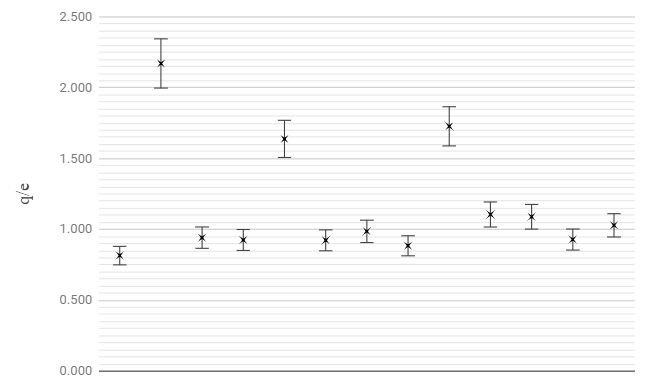
\includegraphics[width=\textwidth]{graph1.PNG}
    \caption{Отношение зарядов капель к заряду электрона}
    \label{fig:vac}
\end{figure}
 
\end{enumerate}

\section{Вывод}

В ходе работы методом масляных капель был экспериментально определён заряд электрона. Точность измерений на предложенной установке позволила определить эту величину с достаточно большой точностью. В основном исследовались капли с зарядами, по модулю равном элементарному. Было и несколько капель с зарядом, по модулю равным $2e$ - полученные для них значения заряда не совсем совпадают с конкретной величиной $2e$, у двух капель он меньше (но больше $e$). Это можно объяснить тем, что при взаимодействии капель друг с другом заряды на них могут перераспределяться, и в течение одного опыта (примерно 5 минут) могло произойти такое взаимодействие и заряд капли изменился. \par
В целом, эксперимент можно считать удачным, так измеренные значения зарядов совпали с зарядом электрона, и значения погрешностей не слишком велики.
\end{document}







